\documentclass{beamer}

\usepackage{xcolor}
\usepackage{graphicx}
\usepackage{varwidth}
% \usepackage{caption}

\usepackage{subcaption}
\usepackage{media9}
\usepackage{multimedia}

\definecolor{NvidiaGreen}{RGB}{118, 185, 0}

\usetheme{Madrid}
\setbeamertemplate{navigation symbols}{}

% Set the colors for various Beamer elements
\setbeamercolor{title}{fg=black, bg=NvidiaGreen} 
\setbeamercolor{frametitle}{fg=black, bg=NvidiaGreen} 
\setbeamercolor{item}{fg=black, bg=NvidiaGreen} 
\setbeamercolor{section in toc}{fg=black, bg=NvidiaGreen}
\setbeamercolor{author}{fg=white, 
        % bg=NvidiaGreen
    }
\setbeamercolor{date}{fg=white, 
        % bg=NvidiaGreen
    }

% Set the background to white for a clean presentation
\setbeamercolor{background canvas}{bg=white}

% #########################################################################################
% #########################################################################################
% Title
% #########################################################################################
% #########################################################################################

\begin{document}
{
\setbeamertemplate{background} 
{
    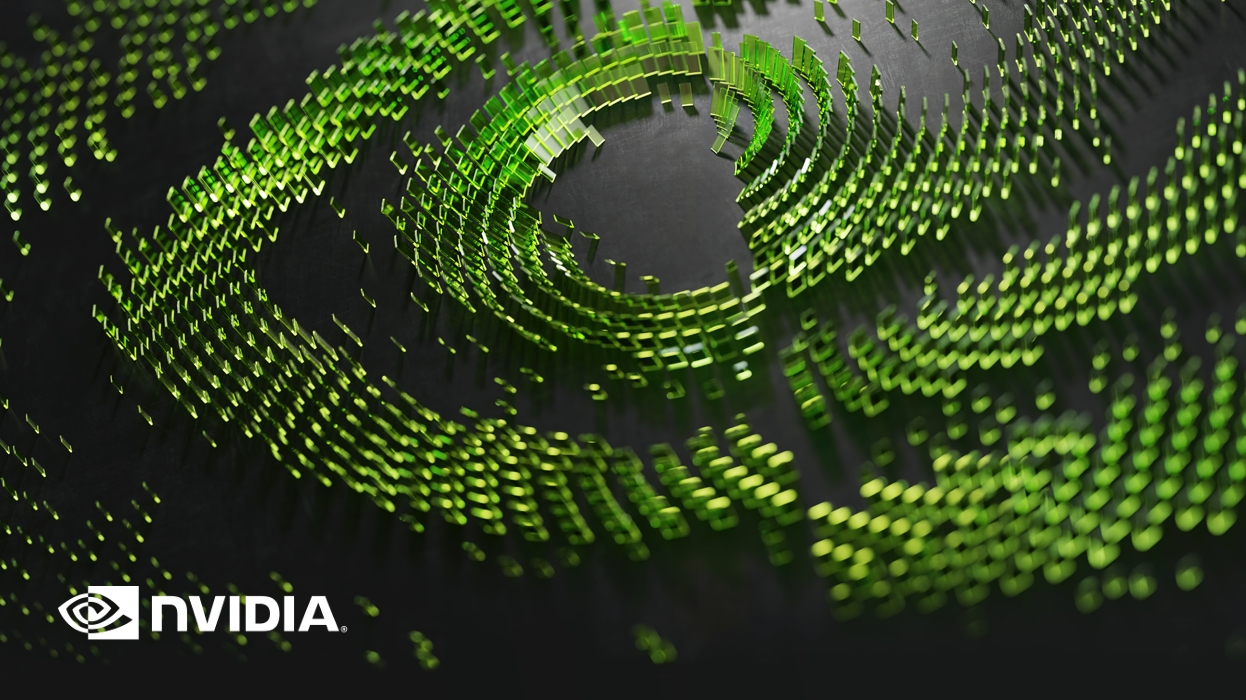
\includegraphics[width=\paperwidth,height=\paperheight]{images/Screenshot_9-12-2024_212019_.jpeg}
}
\title{\textbf{Towards Embodied Intelligence, A Comprehensive review of Computer Vision Architectures}}
\author[]{\textbf{Renan Monteiro Barbosa}}
% \date{\today}
\date[]{\textbf{2024}}
\maketitle
}

% #########################################################################################
% #########################################################################################
% Slide 1 - Advances in Visual Recognition
% #########################################################################################
% #########################################################################################

\section{Advances in Computer Vision}
\begin{frame}
\frametitle{\textbf{Advances in Computer Vision}}
\centering
\begin{minipage}{0.3\textwidth}
    \centering
    \includegraphics[width=\textwidth]{example-image-a} % Replace with your image file
    \captionof{figure}{Title of Image 1}
\end{minipage}
% \hfill
\hspace{0.05\linewidth}
\begin{minipage}{0.4\textwidth}
    \centering
    
\includegraphics[width=\textwidth]{images/imagenet.jpeg} % Replace with your image file
    \captionof{figure}{Bigger Data}
\end{minipage}

\vskip 1em % Adds vertical space between the rows of images

% Second row of images
\centering
\begin{minipage}{0.3\textwidth}
    \centering
    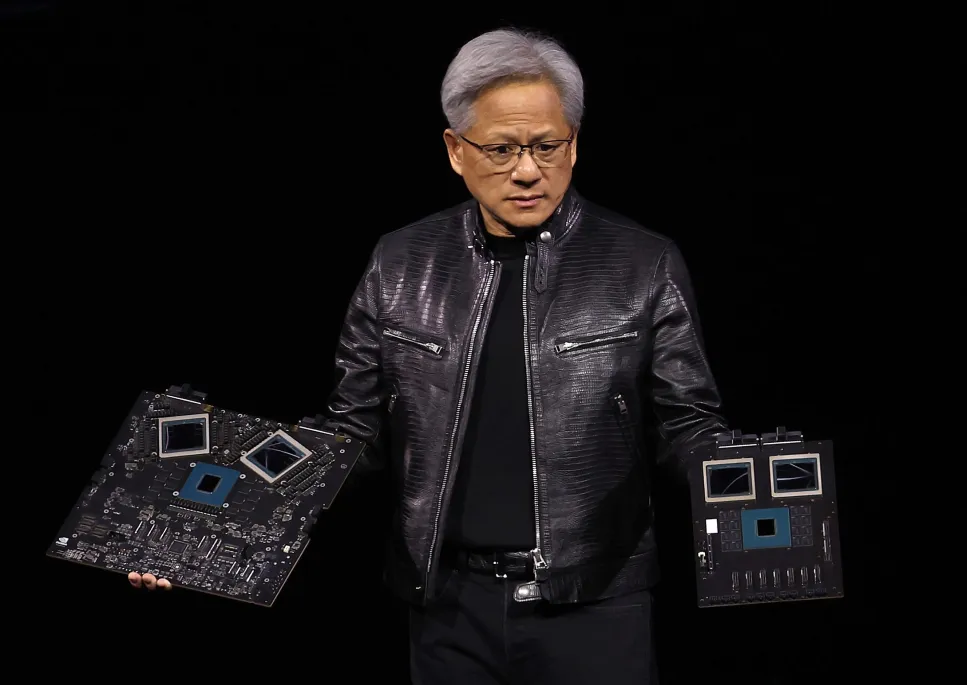
\includegraphics[width=\textwidth]{images/faster-GPUs.png} % Replace with your image file
    \captionof{figure}{Faster GPUs}
\end{minipage}
% \hfill
\hspace{0.05\linewidth}
\begin{minipage}{0.4\textwidth}
    \centering
    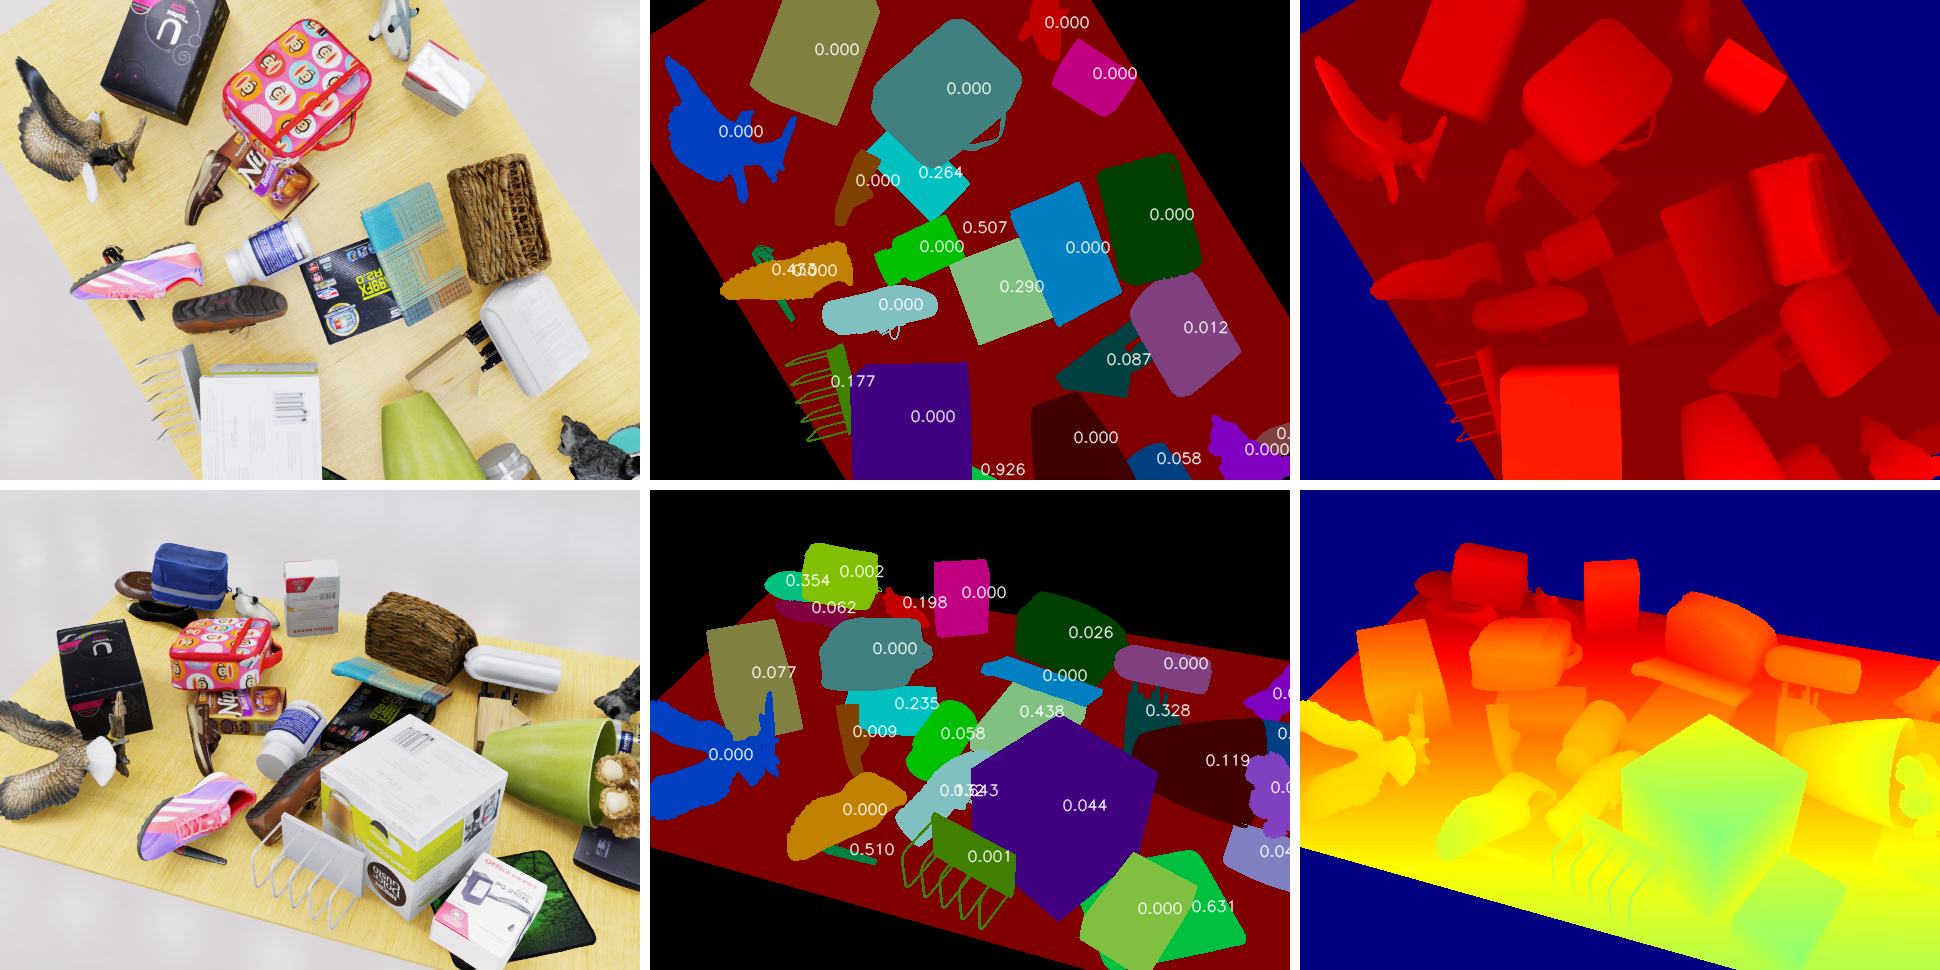
\includegraphics[width=\textwidth]{images/train_data_vis.png} % Replace with your image file
    \captionof{figure}{More powerful models}
\end{minipage}

\end{frame}

% #########################################################################################
% #########################################################################################
% Slide 2 - Real World Data is Imperfect
% #########################################################################################
% #########################################################################################

\section{Real World Data is Imperfect}
\begin{frame}
\frametitle{\textbf{Real World Data is Imperfect}}
\centering
\begin{minipage}{1\textwidth}
    \centering
    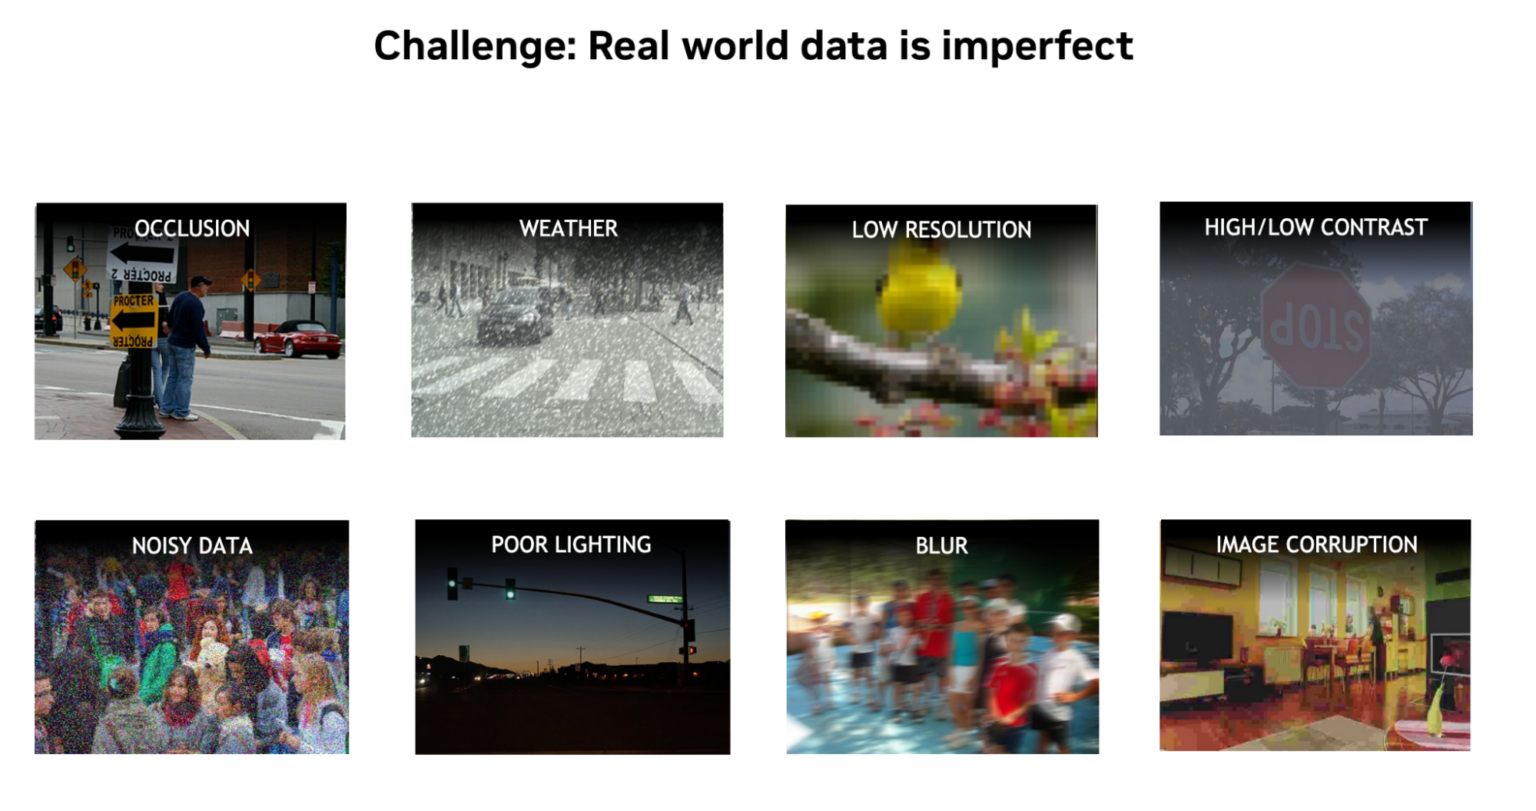
\includegraphics[width=\textwidth]{images/noisy-real-world-data--1536x811.png} % Replace with your image file
    \captionof{figure}{Different types of imperfect and noisy real-world data create challenges for image analysis.}
\end{minipage}
\end{frame}

% #########################################################################################
% #########################################################################################
% Slide 3 - Introduction
% #########################################################################################
% #########################################################################################

\section{Introduction}
\begin{frame}
\frametitle{\textbf{Introduction}}
In recent years, computer vision (CV) has made significant strides in performance due to advancements in deep learning models. This presentation covers the evolution of CV models, starting with YOLO (You Only Look Once) and moving towards Vision Transformers (ViT).

\end{frame}

% #########################################################################################
% #########################################################################################
% Slide 4 - YOLO: You Only Look Once
% #########################################################################################
% #########################################################################################

\section{YOLO: You Only Look Once}
\begin{frame}
\frametitle{\textbf{YOLO: You Only Look Once}}
\begin{itemize}
    \item Introduced by Redmon et al. in 2016, YOLO is a real-time object detection system.
    \item YOLO performs both object localization and classification in a single forward pass of the network.
    \item Significantly faster than previous models, making it ideal for real-time applications.
    \item The architecture is a single convolutional neural network (CNN) that predicts bounding boxes and class probabilities directly from image pixels.
\end{itemize}

\end{frame}

% #########################################################################################
% #########################################################################################
% Slide 5 - YOLO Architecture
% #########################################################################################
% #########################################################################################

\section{YOLO Architecture}
\begin{frame}
\frametitle{\textbf{YOLO Architecture}}
\begin{itemize}
    \item YOLO divides the input image into a grid.
    \item Each grid cell predicts bounding boxes, confidence scores, and class probabilities.
    \item The model outputs a fixed number of bounding boxes, each with a class label and confidence score.
    \item YOLO's speed and accuracy led to its widespread adoption in applications like self-driving cars, security systems, and robotics.
\end{itemize}

\end{frame}

% #########################################################################################
% #########################################################################################
% Slide 6 - 
% #########################################################################################
% #########################################################################################

\section{The Evolution of YOLO}
\begin{frame}
\frametitle{\textbf{The Evolution of YOLO}}
\begin{itemize}
    \item YOLOv1 (2016): The first version, accurate but struggled with small objects.
    \item YOLOv2 (2017): Improved performance by using batch normalization and anchor boxes.
    \item YOLOv3 (2018): Further improvements with multi-scale predictions and better backbone architecture (Darknet-53).
    \item YOLOv4 (2020): Introduced improvements like CSPDarknet53 and additional optimizations for better accuracy and speed.
    \item YOLOv5: A community-driven implementation, offering enhanced performance.
\end{itemize}
\end{frame}

% #########################################################################################
% #########################################################################################
% Slide 1 - 
% #########################################################################################
% #########################################################################################

\section{The Rise of Transformers in CV}
\begin{frame}
\frametitle{The Rise of Transformers in Computer Vision}
\begin{itemize}
    \item Transformers, originally developed for NLP tasks, have revolutionized computer vision in recent years.
    \item Vision Transformers (ViT) are a new architecture that applies the transformer model to image data.
    \item ViT treats an image as a sequence of patches, similar to how transformers treat sequences of words in NLP.
    \item This shift represents a move away from the convolutional layers typically used in traditional CV models.
\end{itemize}
\end{frame}

% #########################################################################################
% #########################################################################################
% Slide 1 - 
% #########################################################################################
% #########################################################################################

\section{Vision Transformer (ViT)}
\begin{frame}
\frametitle{Vision Transformer (ViT)}
\begin{itemize}
    \item Introduced by Dosovitskiy et al. in 2020.
    \item The input image is split into non-overlapping patches (e.g., 16x16 pixels).
    \item Each patch is flattened into a vector and treated as a "token" similar to words in NLP.
    \item These tokens are fed into the transformer encoder to learn the global context of the image.
    \item ViT demonstrated superior performance over traditional CNNs when trained on large datasets like ImageNet.
\end{itemize}
\end{frame}

% #########################################################################################
% #########################################################################################
% Slide 1 - 
% #########################################################################################
% #########################################################################################

\begin{frame}
\frametitle{ViT Architecture}
\begin{itemize}
    \item \textbf{Patch Embedding:} The image is divided into fixed-size patches.
    \item \textbf{Position Encoding:} Since transformers do not have inherent inductive biases for spatial locality, positional encodings are added to capture spatial relationships.
    \item \textbf{Transformer Encoder:} ViT uses the standard transformer architecture, consisting of multi-head self-attention layers.
    \item \textbf{Classification Head:} A final classification token is used to predict the output class.
\end{itemize}
\end{frame}

% #########################################################################################
% #########################################################################################
% Slide 1 - 
% #########################################################################################
% #########################################################################################

\section{Comparing YOLO and ViT}
\begin{frame}
\frametitle{Comparing YOLO and ViT}
\begin{itemize}
    \item \textbf{YOLO:}
        \begin{itemize}
            \item Optimized for real-time object detection.
            \item Excellent for applications requiring speed and efficiency.
            \item Uses CNNs and grid-based predictions for object localization and classification.
        \end{itemize}
    \item \textbf{ViT:}
        \begin{itemize}
            \item A new paradigm that excels in image classification and recognition.
            \item Requires large datasets and computational power for training.
            \item Uses transformers to capture global context, offering flexibility and scalability.
        \end{itemize}
\end{itemize}
\end{frame}

% #########################################################################################
% #########################################################################################
% Slide 1 - 
% #########################################################################################
% #########################################################################################

\section{Applications and Future Directions}
\begin{frame}
\frametitle{Applications and Future Directions}
\begin{itemize}
    \item \textbf{YOLO Applications:}
        \begin{itemize}
            \item Real-time object detection in video streams, surveillance, and autonomous vehicles.
            \item Medical image analysis.
        \end{itemize}
    \item \textbf{ViT Applications:}
        \begin{itemize}
            \item Image classification, segmentation, and more advanced tasks.
            \item Future improvements could focus on reducing the need for large datasets.
            \item ViT may extend into multimodal applications (e.g., combining vision and language).
        \end{itemize}
    \item \textbf{Future of Computer Vision:}
        \begin{itemize}
            \item Hybrid models combining CNNs with transformers.
            \item Self-supervised learning to reduce reliance on labeled data.
            \item Expansion into other domains like 3D vision, robotics, and healthcare.
        \end{itemize}
\end{itemize}
\end{frame}

% #########################################################################################
% #########################################################################################
% Slide 1 - 
% #########################################################################################
% #########################################################################################

\section{Conclusion}
\begin{frame}
\frametitle{Conclusion}
The development of computer vision models has progressed rapidly, from YOLO’s fast and efficient real-time object detection to the powerful and flexible Vision Transformers. Both models represent milestones in the field, with YOLO excelling in speed and ViT pushing the boundaries of performance in image recognition. The future of computer vision is bright, with ongoing research promising even more breakthroughs.
\end{frame}

% #########################################################################################
% #########################################################################################
% #########################################################################################
% #########################################################################################

% ⠀⠀⠀⠀⠀⠀⠀⠀⠀⠀⠀⠀⠀⣀⣀⣀⡀⠀⠀⠀⠀⠀⠀⠀⠀⠀
% ⠀⠀⠀⠀⠀⠀⢀⣠⠤⠖⠈⠉⠉⠀⠀⠀⠀⠉⠢⡀⠀⠀⠀⠀⠀⠀
% ⠀⠀⠀⠀⠀⣴⠏⠀⠀⠀⠀⠀⠀⠀⠀⠀⠀⠀⠀⠈⢦⡀⠀⠀⠀⠀
% ⠀⠀⠀⣠⠞⠁⠀⠀⠀⠀⠀⠀⠀⠀⠀⢀⠞⠋⢙⣦⡈⣷⡄⠀⠀⠀
% ⠀⣀⠶⠁⠀⠀⣀⣀⡀⠀⠀⠀⠀⠀⡴⠁⠀⠀⠿⢿⡟⣌⢿⠀⠀⠀
% ⣠⡿⠀⢠⣜⠉⠀⠀⠙⢷⢄⠀⠀⠀⢧⠀⠀⠀⠀⠀⠀⠘⡆⢧⡀⠀
% ⣯⠃⠀⢾⣿⠗⠀⠀⠀⠀⡽⠀⠀⠀⠈⠳⢄⣀⠀⠀⠀⡰⠃⠘⣵⡄
% ⡏⠀⠀⠘⡄⠀⠀⠀⣠⠞⠁⠀⠀⠀⠀⠀⠀⠀⠉⠉⠁⠀⠀⠀⢱⡇
% ⡅⠀⠀⠀⠙⠒⠔⠚⠁⠀⠀⠀⠀⠀⠀⠀⠀⠀⠀⠀⠀⠀⠀⠀⠀⡇
% ⣧⡀⠀⠀⠀⠀⠀⠀⠀⠀⠀⠀⠀⠀⠀⠀⠀⢠⠀⠀⠀⠀⠀⠀⠀⡗
% ⡿⡇⠀⠀⠀⠀⠀⠀⠀⠀⠀⢠⡀⠀⠀⠀⠀⢸⡇⠀⠀⠀⠀⠀⠀⣇
% ⠹⣷⠀⠀⠀⠀⠀⠀⠀⠀⠀⠈⠷⣤⣤⣤⣤⠞⠁⠀⠀⠀⠀⠀⠀⣸
% ⠀⠸⣇⠀⠀⠀⠀⠀⠀⠀⠀⠀⠀⠀⠀⠀⠀⠀⠀⠀⠀⠀⠀⠀⣰⠇
% ⠀⠀⢇⠳⣄⠀⠀⠀⠀⠀⠀⠀⠀⠀⠀⠀⠀⠀⠀⠀⠀⠀⠀⢀⡏⠀
% ⠀⠀⠈⠀⠀⠉⠀⠀⠀⠀⠀⠀⠀⠀⠀⠀⠀⠀⠀⠀

% #########################################################################################
% #########################################################################################
% #########################################################################################
% #########################################################################################

\end{document}